\documentclass[12pt]{article}
\pdfoutput=1

\usepackage[T1]{fontenc}
\usepackage{verbatim}
\usepackage{float}
\usepackage{amsthm}
\usepackage{amsmath}
\usepackage{amssymb}
\usepackage{graphicx}
\usepackage{color}
\usepackage{url}
\usepackage{caption}
\usepackage{subcaption}
\usepackage{mathtools} 
\usepackage{stackrel} 

\newcommand{\LL}{\mathcal{L}}
\newcommand{\E}{\mathbb{E}}
\newcommand{\I}{\mathcal{I}}
\newcommand{\ep}{\varepsilon}
\newcommand{\Z}{\mathbb{Z}}
\newcommand{\GCD}{\mathbf{GCD}}
\newcommand{\XX}{\mathcal{X}}
\newcommand{\SUM}{\text{sum}}
\newcommand{\1}{\mathbf{1}}
\newcommand{\rr}{\textbf{r}}
\newcommand{\ii}{\textbf{i}}
\newcommand{\jj}{\textbf{j}}
\newcommand{\Poisson}{\text{Poisson}}
\newcommand{\II}{\mathcal{I}}
\newcommand{\kk}{\textbf{k}}
\newcommand{\RR}{\mathbb{R}}
\newcommand{\mb}{\mathbf}
\newcommand{\mk}{\mathfrak}
\newcommand{\mc}{\mathcal}
\newcommand{\TODO}[1]{{\color{red}{[#1]}}}
\newcommand{\revised}[1]{{\color{magenta}{#1}}}
\newcommand{\R}{\mathbb{R}}
%\newcommand{\M}{\mathcal{M}}
\newcommand{\M}{m}
\renewcommand{\P}{\mathbb{P}}
\renewcommand{\L}{\mathcal{L}}

\makeatletter

\newcommand{\reals}{\mathbb{R}}
\newcommand{\RL}{\mathbb{R}^L}
\newcommand{\tamir}{x}
\newcommand{\CL}{\mathbb{C}^L}
\newcommand{\RN}{\mathbb{R}^N}
\newcommand{\RNN}{\mathbb{R}^{N\times N}}
\newcommand{\RPP}{\mathbb{R}^{P\times P}}
\newcommand{\CNN}{\mathbb{C}^{N\times N}}
\newcommand{\inner}[1]{\left\langle {#1} \right\rangle}
\newcommand{\hx}{\hat{x}} 
\newcommand{\one}{\mathbf{1}} 
\newcommand{\be}
{\begin{equation}}
\newcommand{\ee}
{\end{equation}}
%\renewcommand{\P}{\mathbb{P}}
\newcommand{\aseq}{\stackrel{a.s.}{=}}
\renewcommand{\P}{\mathrm{Prob}}


\theoremstyle{plain}
\newtheorem{thm}{\protect\theoremname}[section]
\theoremstyle{definition}
\newtheorem{defn}[thm]{\protect\definitionname}
\theoremstyle{remark}
\newtheorem{claim}[thm]{\protect\claimname}
\theoremstyle{plain}
\newtheorem{lem}[thm]{\protect\lemmaname}
\newtheorem*{lem*}{Lemma}
\theoremstyle{remark}
\newtheorem{rem}[thm]{\protect\remarkname}
\theoremstyle{plain}
\newtheorem{corollary}[thm]{\protect\corollaryname}
\theoremstyle{plain}
\newtheorem{conjecture}[thm]{\protect\conjecturename}
\theoremstyle{plain}
\newtheorem{proposition}[thm]{\protect\propositionname}
\providecommand{\claimname}{Claim}
\providecommand{\definitionname}{Definition}
\providecommand{\lemmaname}{Lemma}
\providecommand{\remarkname}{Remark}
\providecommand{\theoremname}{Theorem}
\providecommand{\corollaryname}{Corollary}
\providecommand{\propositionname}{Proposition}
\providecommand{\conjecturename}{Conjecture}

\usepackage{authblk}
\renewcommand*{\Affilfont}{\normalsize}
\setlength{\affilsep}{2em}   % set the space between author and affiliation

\usepackage[margin=3cm]{geometry}

\allowdisplaybreaks
\numberwithin{equation}{section}


\RequirePackage[colorlinks,citecolor=blue,urlcolor=blue,linkcolor=blue]{hyperref}


\begin{document}

%\begin{frontmatter}


\title{Response to referees: Multi-target detection with application to cryo-electron microscopy}

\author{Tamir Bendory, Nicolas Boumal, Will Leeb, Eitan Levin, and Amit Singer}

\date{}
\maketitle

We thank the editor and the referees for their comments on our paper. Below, we provide a detailed, one-to-one response to all comments. 

\section{Referee 1}

\noindent \textbf{Comment:} The only suggestion I have is to include a brief discussion of validation - the experiments here are from simulated data with known signals. If this technology were ever to be adopted in experimental practice, some form of statistical validation will be essential.\\

\noindent \textbf{Response:} We agree that statistical validation is important, in particular for single particle reconstruction using cryo-EM. %This question is more general that the specific method applied.
Several heuristics are used in cryo-EM. A common one is to split the data into two halves, reconstruct two structures independently, then compare them. 
It is easy to apply the same technique to our framework. We added a few sentences to this effect in the numerical experiments section.
 
%Unfortunately,  there is  no rigorous method to validate a structure that was constituted using cryo-EM. In practice, researchers in the field use several useful heuristics, such as  comparing the elucidated structure with structures that were reconstructed by other imaging modalities (e.g., X-ray crystallography), or different statistical techniques (e.g., expectation-maximization). The validation problem is even more severe in the low SNR regime (the main interest of this paper) in which visual assessment of the data might be impossible. Our method does not offer insights for this question.

%While validation is beyond the scope of this paper, autocorrelation analysis provides a flexible framework to describe reach generative models of the data. We added a paragraph in the summary to explain this issue. 
 
%\TODO{Split the data into to halves independently and compare; checking objective and flexible model; analysis from optimization perspective of the LS } 

\section{Referee 3}

\noindent \textbf{Comment:} An important point in practical image reconstruction, especially in modalities like phase retrieval, is that precise knowledge of the support of the image makes the reconstruction problem considerably easier.  Beyond that, having an image with a sharply delineated, known boundary is, in fact, a huge advantage. Such images are used in the examples in this paper, along with an exact knowledge of their support.  In most realistic imaging applications such information is not available, and this renders these problems inherently more difficult, regardless of the algorithm used. Some mention of this fact should appear in this paper.\\

\noindent \textbf{Response:} Section 4.4 discusses the application of our approach to 2-D images. For Einstein's image used in the manuscript, the boundary of the second-order autocorrelation  can be identified easily if the second-order autocorrelation is known precisely (that is, $N\to\infty$); see Figure~\ref{fig:XC} (in this report). 
Since the image is square, it implies the support of the image itself. 
In Section 4.4, we underscore the importance of the knowledge of the exact support for phase retrieval (recovery from second-order autocorrelation) as was shown in [9]. 
We revised a couple of sentences in this section for the sake of clarity. 

If exact support knowledge is not available, our proposed solution is to consider the third-order autocorrelation.
To demonstrate it, in the revised manuscript, we changed Experiment 1. Now, half of the first signal in Figure 1 is zero, which allows us to simulate the situation in which the support of the signal is overestimated. Our algorithm still recovers the signal accurately. \\

\begin{figure}[h]
	\centering
	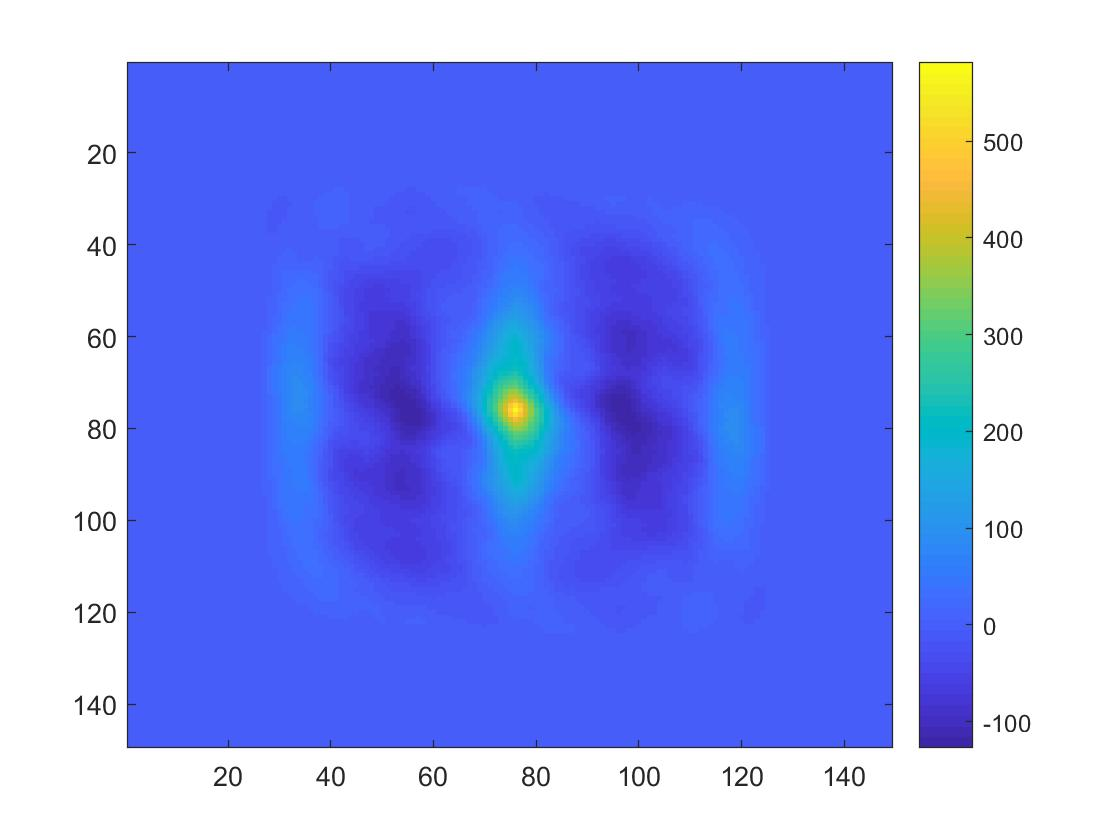
\includegraphics[scale=0.3]{Xcorr}
	\caption{	\label{fig:XC} The second-order autocorrelation of Einstein's image used in the paper (padded by zeros).}
\end{figure}

\noindent \textbf{Comment:} Though it is clarified in the proof of Prop. 4.5 it is not immediately clear that  the right hand sides of formulae (4.3), (4.4), (4.5) are observable quantities. A remark, after the statement of the proposition, clarifying this  point would be useful.\\

\noindent \textbf{Response:} We added a remark to the proposition to make this point clear.\\

\noindent \textbf{Comment:}  I found it difficult to understand what Figure 2 is demonstrating. Perhaps it is a result of the poor rendering of the grey-scale.
\\ 

\noindent \textbf{Response:} The number of autocorrelation entries we compute increases with the signal length $L$. Hence, we expect that, as $L$ grows, we should be able to estimate more and more distinct signals in the heterogeneous case. The experiment reported in Figure 2 illustrates how $K$ (the number of signals we can estimate simultaneously) grows as a function of $L$. Since to do the actual recovery we need to solve a non-convex optimization problem, this experiment is setup so that we can distinguish between the effects of statistical and computational difficulties.

We find this figure important to inspect (empirically) how many signals can be estimated simultaneously from a mix of their autocorrelations. We agree that this figure should be visualized in a colored version of the manuscript. We used a similar figure for the same purpose (but for a different problem) in a previous publication: Boumal, N., et al. ``Heterogeneous multireference alignment: A single pass approach.'' \emph{2018 52nd Annual Conference on Information Sciences and Systems (CISS)}. IEEE, 2018.



\end{document}


